% =============================================================================
% From Revert to Remedy: Process Modeling Wikipedia's Dispute Escalation
% University of Virginia School of Data Science - Capstone, 2026
%
% IEEE Conference Template (IEEEtran).
% On Overleaf: create a new project, paste this into main.tex, set the
% compiler to pdfLaTeX, and Recompile. The bibliography stu-b at the bottom
% uses BibTeX (.bib file).
% =============================================================================
\documentclass[conference]{IEEEtran}
\IEEEoverridecommandlockouts
% The preceding line is only needed to identify funding in the first footnote. If that is unneeded, please comment it out.
\usepackage{cite}
\usepackage{amsmath,amssymb,amsfonts}
\usepackage{algorithmic}
\usepackage{graphicx}
\usepackage{textcomp}
\usepackage{xcolor}
\usepackage{url}
\usepackage{hyperref}
\usepackage[inkscapelatex=false]{svg}
\usepackage{booktabs}
\hypersetup{
    colorlinks=true,
    linkcolor=blue,
    citecolor=blue,
    urlcolor=blue
}
\def\BibTeX{{\rm B\kern-.05em{\sc i\kern-.025em b}\kern-.08em
    T\kern-.1667em\lower.7ex\hbox{E}\kern-.125emX}}
\begin{document}

\title{From Revert to Remedy:\\
       Process Modeling Wikipedia’s Dispute Escalation}

\author{\IEEEauthorblockN{Louis Cocks}
\IEEEauthorblockA{\textit{School of Data Science} \\
\textit{University of Virginia}\\
Charlottesville, VA, USA \\
epx8hh@virginia.edu}
\and
\IEEEauthorblockN{Katherine Kelleher}
\IEEEauthorblockA{\textit{School of Data Science} \\
\textit{University of Virginia}\\
Charlottesville, VA, USA \\
kbk8vh@virginia.edu}
\and
\IEEEauthorblockN{Ryan Healy}
\IEEEauthorblockA{\textit{School of Data Science} \\
\textit{University of Virginia}\\
Charlottesville, VA, USA \\
rah5ff@virginia.edu}
}

\maketitle

\begin{abstract}
The objective of this project is the development of an automated framework for extracting formal ontologies and generating clear, executable process models from Wikipedia disputes. This research addresses the challenge of translating raw Wikipedia disputes into machine-readable representations that visualize dispute workflow representation and provide insight into the differences between stated and actual processes. By providing Wikipedia users and admin an analysis of dispute data and deterministic business process models, these stakeholders will have a better understanding of arbitration and other dispute cases. This information can be used to revise or enhance existing dispute processes.
\end{abstract}

\begin{IEEEkeywords}
Wikipedia, Business Process Model \& Notation (BPMN), dispute resolution noticeboard (DRN), Arbitration (Arb), Request for Comment (RfC), edit wars, collaborative governance, escalation prediction, MediaWiki Application Programming Interface (API), Bidirectional encoder representations from transformers (BERT), Named Entity Recognition (NER).
\end{IEEEkeywords}

% =============================================================================
\section{Introduction \& Motivation}
% =============================================================================
This project demonstrates the use of Ontology Extraction and Business Process Modeling \& Notation (BPMN) within the domain of the Wikipedia arbitration processes. The objective is to extract processes for Wikipedia disputes of any kind, including arbitration cases, dispute resolution noticeboards (DRN), and requests for comment (RfC), by gathering documentation, extracting and mining data, and using subject matter expertise to verify processes.

In practice, this project (1) provides Wikipedia users with clarity on the various avenues in which disputes are often handled and (2) demonstrates a proof-of-concept analytical solution that can be generalized and used to extract process information. The models produced for this project can help distill the complicated nuances of varied Wikipedia dispute processes, typically only known by Wikipedia experts, by visually representing processes as sequences of formal or informal events. The proof-of-concept solution and methodology for process extraction from extensive text data can provide value by demonstrating how a technical solution collects and analyzes information at scale, providing insight into processes that would otherwise be manually intensive or impossible to interpret without domain expertise.

% =============================================================================
\section{Background}
% =============================================================================

Wikipedia's dispute-resolution process has evolved substantially over more than two decades. The English Wikipedia adopted its first formal arbitration mechanism in 2003, when project co-founder Jimmy Wales delegated authority over complex conduct cases to a community-elected Arbitration Committee (ArbCom) in response to a volume of disputes that he could no longer personally adjudicate ~\cite{b1}. In subsequent years, various ancillary stages have existed and been deprecated such as the now-defunct Mediation Committee, Wikiquette Assistance, and the Association of Members' Advocates, among others. These forums, as well as established stages such as the Dispute Resolution Noticeboard (DRN) and structured Requests for Comment (RfC), comprise parts of a graduated-intervention pathway which may be invoked in different combinations as part of a Wikipedia arbitration process\cite{b2, b3}.

Empirical research has characterized the distinct dynamics of conflict on Wikipedia: Yasseri, Sumi, Rung, Kornai, Kertész identified three developmental patterns for controversial articles and showed that edit wars are typically waged between small numbers of editors in strong disagreement ~\cite{b4}. A more recent political-science scholarship argued that Wikipedia's content has been shaped less by formal rules than by the resolution of early ambiguous disputes in which interpretations of policies such as "Neutral Point of View" carried institutional force~\cite{b5}. Despite these bodies of work, studies do not produce an executable, role-aware process model of how a dispute moves through Wikipedia's full multi-stage resolution pathway, which is addressed in this paper.

Comparative work has shown that BPMN models typically use roughly 40\% fewer elements than equivalent event-driven process chains~\cite{b6}, and the standard's swimlane construct is well suited to procedures with explicit role boundaries. These characteristics align to the use case of modeling the structure of Wikipedia's tiered dispute-resolution system, which involves volunteer mediators, administrators, and elected arbitrators. BPMN has been applied extensively to enterprise workflows, healthcare pathways, and public-sector procedures and has the potential to be extended to online-platform governance. BPMN provides a standardized vocabulary and the ability to represent case-specific branching for Wikipedia disputes that traverse multiple stages, multiple actors, and multiple decision gateways before reaching closure. Wikipedia's dispute resolution process has evolved over time, but available stages are well documented and many of the key and significant stages have historically remained the same. Thus, translating a single case page into a process model is not a process discovery problem ~\cite{b7}, as the procedural stages are already documented and relatively stable. The task of this paper is content extraction at scale: determining which procedural branches a case followed, accounting for variation in sequence, identifying the actors involved, and linking the relevant policies and evidence cited.

% =============================================================================
\section{Data Description}
% =============================================================================
Wikipedia's dispute-resolution venues, including the Arbitration Committee (ArbCom), the Dispute Resolution Noticeboard (DRN), and Requests for Comment (RFC) pages operate as well-defined venues for adjudication and/or deliberation. These webpages have case records that are recorded as semi-structured wikitext and are the focus of this paper.

\subsection{Source APIs}
% MediaWiki, ORES, Pageviews, XTools
The raw data documented and analyzed are sourced from available open-source Wikimedia APIs. In particular, the information sourced from Wikipedia APIs is unstructured data related to informal and formal stages of the Wikipedia dispute resolution process. Several Python scripts systematically retrieve data and pull information about key process stages from "MediaWiki" APIs directly and via a wrapper "WikiClient" for Pywikibot. These APIs are also used to collect text lineage for arbitation cases using depth-first search to link case history.

Arbitration case history includes the following relevant variables:
\begin{itemize}
    \item Case Opening/Closing date
    \item Relevant parties
    \item Confirmation that all parties are aware of the request
    \item Other attempted steps in dispute resolution
    \item Requests for comment
    \item Statements
    \item Preliminary decisions
    \item Consequences
\end{itemize}

\subsection{Corpus Composition}
More than 70 MB of data was pulled for this project, including Arbitration Case pages submitted to ArbCom, DRN, and RfC posts. There were 485 arbitration cases analyzed, more than 3,000 DRN cases, and about 600 RFC pages with cases covering disputes from 2009 to 2026.

\subsection{Data Assumptions and Limitations}
Some data assumptions are made for the purposes of the analysis of this project:
\begin{itemize}
    \item Lineage extraction from the arbitration process cannot account for dead links or a change in the host of a webpage.
    \item This project cannot fully validate with perfect accuracy whether the text data represent the true events and full scope of real-life, Wikipedia arbitration processes, and disputes.
    \item To maintain scope and scalability, no personal individual information about users within a dispute is considered in scope for this project.
\end{itemize}

Due to the nature of Wikipedia dispute and arbitration data, the following limitations will affect the results of this project:
\begin{itemize}
    \item Running BPMN and visualizing at scale may result in process abstraction.
    \item Cleaning diverse unstructured data formats often requires subject matter expertise or expensive infrastructure, thus automating a generic solution for process extraction must account for scaling costs.
    \item The available data represents Wikipedia dispute processes from more than 20 years of data, likely reflecting an evolving process over time when comparing temporarily distance cases.
\end{itemize}\

For computational power and memory purposes, the University of Virginia’s Rivanna (high-performance computing (HPC) cluster) is utilized to pull a complete data set using a slurm-script that contains all revisions of the RfC, Edit War, DRN, and Arbitration pages.


% =============================================================================
\section{Methodology}
% =============================================================================

\subsection{Data Collection and Cleaning}
Initial data processing involves cleaning unstructured text into a semi-structured format, aligning to the general, commonly used Wikipedia dispute templates.

\subsection{Data Analysis}
To extract processes from natural language documents, several models were considered. The first is natural language processing (NLP) models such as Regex based Text-to-BPMN, which supports process extraction with coded logic and procedural rules based on textual references to known events in the arbitration process. This project evaluated the technique using domain expertise and a cross-comparison of three different modeling pathways. These techniques, one of which includes a common large-language model, are assessed for their utility and ability to perform process extraction with a few arbitration cases. A few cases are validated by a subject-matter-expert for references to arbitration stages, with focus on minimizing false positives and maximizing precision to prioritize accurately modeling events.

The resulting models generated for this project are rendered in BPMN 2.0 format for comprehension of the widest possible audience and in support of Wikipedia's role-based procedural design; its standardized vocabulary of activities, gateways, and events allows the same diagram to be opened in any modeler that can read .bpmn without bespoke tooling. Three modeling approaches are outlined below that address the problem of process extraction in multiple ways.


\subsection{Modeling Target and Extraction Mechanisms}
The core engineering objective of all three modeling approaches is to generate a useful process diagram from extract text that visualizes events, decisions, and involved parties. Wikipedia dispute cases often are documented in long, semi-structured documents that commonly follow a template with case specific details about the case. Many documented arbitration cases contain accepted case evidence, remedies imposed as consequences, and cited Wikipedia policies, often written in narrative prose. A useful process model should represent a narrative sequence of events as discrete BPMN elements rather than collapse the stages of the process into a single "Render decision" task.
Three extraction methodologies were developed for this project, each with different costs, dependencies, and accuracy profiles:
\begin{itemize}
\item deterministic regular expressions (regex)
\item A BERT domain-specific Named Entity Recognition (NER) model from HuggingFace
\item A general-purpose instruction-tuned language model
\end{itemize}\

This project explores multiple methodologies for generating BPMN output to evaluate their strengths and weaknesses. These approaches are assessed against the same set of validation cases (mostly the Abortion case, which produces a long life cycle with multiple amendments and clarifications). The discussion in the following describes each approach, their strengths, and limitations.

\subsubsection{Regex Deterministic Structural Extraction}
The first modeling approach targets ArbCom, DRN, and RfC cases separately, supplied as a pre-fetched JSON corpus. The method relies upon stable section-level structure common to ArbCom case pages, such as Involved parties, Principles, Findings of fact, Remedies, and Enforcement. These reliable structural facts are extracted by regular expression. The Section-level regex is used to identify the counts of proposed principles, findings, and remedies. Additional regex is used to parse the open and closed dates of the case, the list of involved-parties, and the votes on the case decisions. Finally, an outcome heuristic classifies the case as "Declined," "Closed-No-Decision," "Admonishment-Only," or "Remedies-Imposed" using keywords detected in the remedy section.

A custom SwimlaneBpmnBuilder class in the code then generates BPMN 2.0 XML outputs with full Diagram Interchange (DI) coordinates. The four-lane layout, including the roles "Requesting Party", "Clerk," "Arbitrators," and "Enforcement," represent distinct procedural roles in rows that are critical to understanding the process. This method produces structurally valid and readable diagrams without model dependencies, significant GPU, or rate-limited inference. Its limitation is the rigidity of the approach: the diagrams capture high-level findings aligned to document headers, but fail to capture their content in detail, such as their voting margins, or the specific policies cited.

\subsubsection{Domain-Specific BERT NER}
The second method involves the rule-based strategy of the first, but involves a HuggingFace BERT token-classification model, bpmn-information-extraction, trained specifically to label BPMN-relevant entities\cite{b10}. The model emits five label types: AGENT (person or role), TASK (activity), TASK\_INFO, PROCESS\_INFO, and CONDITION. This method involves chunking long sections at paragraph boundaries to fit the model's 512-token window and runs NER over the case's sections including "Statement by," "Findings of Fact," "Remedies," "Final decision," and "Preliminary" decisions.

Two architectural decisions distinguish this methodology from simply tagging every event or task the model finds. First, the diagram's format remains rule-based: checking for the presence of specific section headings ("RfC," "Preliminary decisions," "Findings of Fact," and an enforcement keyword regex applied to the "Remedies "and "Final Decision" text). It also represents the corresponding optional branches in a fixed BPMN flow. This produces a case-specific shape without trusting the model to reconstruct procedural ordering. Second, the NER output is used narrowly, primarily to populate the enforcement task label with the actual sanction wording recovered from the case ("topic-banned", "blocked"), falling back to a generic label if no enforcement-typed task is found.

This iteration substantially improves the labeling of enforcement actions and surfaces actor entities that the regex pipeline missed, but it is limited in that the BPMN rules are still based on a fixed template, so a case with twelve proposed remedies still renders as one Enforce Remedies task. The number of branches in the resulting diagram does not reflect the number of decisions the committee actually made.

Both Regex Deterministic Structural Extraction and Domain-Specific BERT NER output a .bpmn and custom automated PNG image (via the processpiper library, which avoids a Chromium dependency).

\subsubsection{Hybrid Extraction with Per-Decision Branching}
The final methodology evaluated replaces the fixed rule-based approach based on Wikipedia case templates with a content-driven strategy. This modeling method generalizes the pipeline to support all three venues (Arb, DRN, RfC). It also abandons the BERT NER model in favor of a general-purpose instruction-tuned language model (Google's Gemma 3-4b-it, with optional 4-bit quantization for larger model sizes like the 12B-parameter variant requiring approximately 28 GB of VRAM), prompted to emit structured JSON conforming to a fixed schema. The deterministic regex layer is retained and runs first, supplying ground-truth structural facts (vote tallies, dates, party lists) that the language-model passes consume.

The central design change involves each individual proposed item becoming its own BPMN element. The model runs five focused extraction passes for ArbCom cases to extract principles, findings of fact, remedies, life-cycle (enforcement actions, amendments, appeals, clarifications, post-case motions), and participant identities. Each event or outcome is returned by the model and rendered as a \textit{user task} followed by an exclusive gateway labeled with the actual item name (e.g., "Neutral Point of View passed?"). The branch count of a substantive case rises from the two or three generated by the previous methods to between fifteen and thirty. The Abortion case in  Fig.~\ref{fig:bpmn-Abortion-svg}, for example, produces 15 gateways and 26 tasks across six lanes, with 255 invocations of 64 distinct policies, guidelines, and essays surfaced from the life-cycle text. The lane structure includes a greater number of lanes, expanding to six lanes for "Requesting Party," "Other Editors," "Clerk," "Drafting Arbitrators," "Full Committee," and "Enforcement."

Each arbitration venue, from RfC to ArbCom, has a specific swimlane layout registered in a module-level \textit{VENUES} specification. This reflects the venue's available procedural roles, an ordered list of extraction prompts, and a venue-specific system prompt. DRN cases use a four-lane layout ("Filing Party," "Other Parties," "Volunteer Mediator," "Closer") and three extraction passes covering parties, mediated-discussion structure, and closure type. RfC cases use a three-lane layout ("Proposer," "Participants," "Closer") and three passes covering the proposal, vote distribution, and consensus finding. All three venues use the same custom \textit{SwimlaneBpmnBuilder}, the same regex extractors for rule invocations and name-space links, and the same SVG renderer; only the prompts, lane layouts, and BPMN composition logic differ. These diagrams include a three-column footer panel summarizing element counts, the full set of invoked rules with policy/guideline/essay typing, and the name-space distribution of evidence links, making each diagram self-contained with model and metrics.

Several engineering decisions arise from the computational constraints of available computing power. A VRAM-aware budget function sizes each extraction pass's input window to whatever fits alongside the model weights, halving the input if encountering a CUDA out-of-memory error and retrying. The script accepts four main input modes: single-case fetch by title, batch fetch of an entire DRN archive page, pre-fetched JSON corpora, and arbitrary text files paired with a venue specification. With added functionality of a \textit{--filter-titles} flag, this narrows any JSON corpus to specific cases by substring match for quick filtering of large data sources. Lastly, aggregate mode is venue-segregated, meaning that separate flags read every JSON file in a directory, filter by the embedded venue field, and emit one corpus-level SVG per venue showing additional metrics like outcome percentages, top invoked rules, namespace distributions, and element averages. The aggregate step does not perform language-model inference (milliseconds per run), allowing the corpus diagram to be regenerated each time a case is added.

% =============================================================================
\section{Results: Dashboard and Analysis}
% =============================================================================
\subsection{Analysis Overview}
To display Wikipedia BPMN visualizations, a dashboard was developed, shown in Figure 1. Hosted on Vercel, it displays an overview of the 485 Wikipedia Arbitration Cases at the time of publication. In these cases, over 3,000 unique users are mentioned, and the average duration of a case is about 56.6 days. In Fig.~\ref{fig:Dashboard Overview}, the line graph highlights that ArbCom activity peaked around 2007 to 2009 and has declined steadily since, likely reflecting evolving community norms on Wikipedia and the introduction of alternative dispute mechanisms. The most common remedy verb is "banned," appearing 544 times, which indicates the severity of cases that actually reach the remedy stage. Analysis shows that the most common remedy action referenced in these arbitration cases is “banned." Additionally, the presence of over 20,000 pages that are titled "Wikipedia:" or "WP:," which are pages dedicated to documentation, policies, and guidelines used by editors, indicates that cases commonly involve the citation of process rules and principles.

\begin{figure}[htbp]
\centering
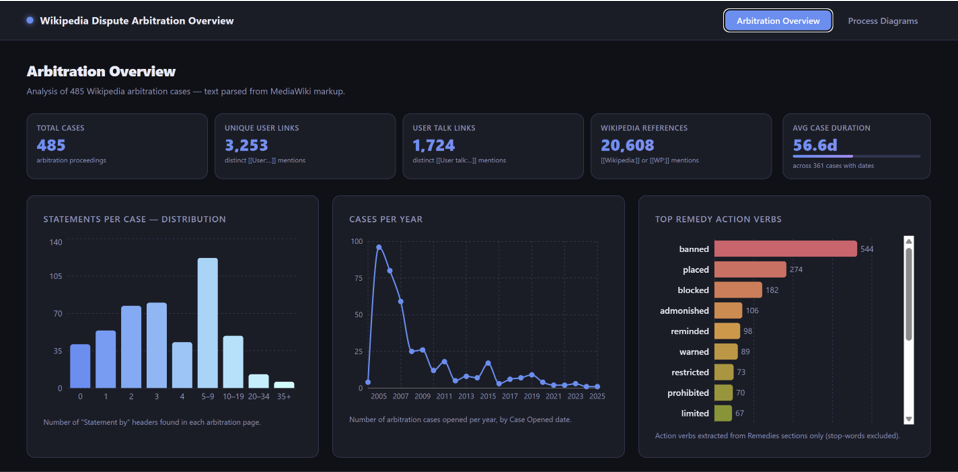
\includegraphics[width=\columnwidth]{Images/Dashboard_overview.png}
\caption{Printed image of the main dashboard arbitration overview screen with relevant metrics.}
\label{fig:Dashboard Overview}
\end{figure}

\subsection{Process Model Validation}
The models developed for this report were validated by a Wikipedia Subject Matter Expert (SME), Lane Raspberry, at the School of Data Science at the University of Virginia. This domain-specific knowledge of Wikipedia disputes and cases provided critical feedback on model outputs and their accuracy. This review included dashboard user testing and a review of individual process diagrams to determine their precision and areas for refinement. To further validate case specific findings, the final analytical solution provided over fifteen metrics such as number of rules invoked, parties, principles, amendments, policies, guidelines, and essays that could be validated directly against Wikipedia page content for correctness. The SME findings indicated that the process diagrams generated with the model were consistent with the textual references found in Wikipedia pages for Arbitration cases \cite{b12}.

\subsection{Aggregate Patterns Across Venues}
We first showcase BPMN from a Regex Deterministic Structural Extraction aggregate.
\begin{figure}[htbp]
\centering
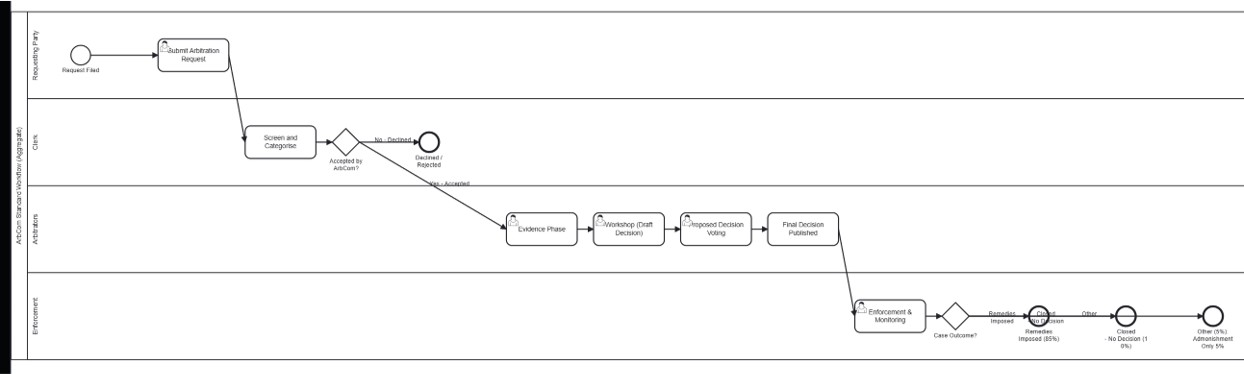
\includegraphics[width=\columnwidth]{Images/BPMN_Aggregate.jpg}
\caption{Extracted process map drafted in BPMN 2.0 file format.}
\label{fig:BPMN-aggregate}
\end{figure}

\begin{figure}[htbp]
\centering
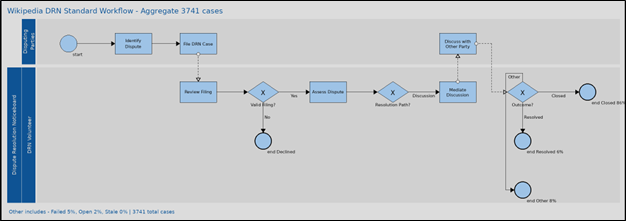
\includegraphics[width=\columnwidth]{Images/BPMN_Aggregate.png}
\caption{Automated PNG output converted from .bpmn file providing additional metrics.}
\label{fig:BPMN-aggregate-png}
\end{figure}

This deterministic rule-based converter method extracts the aggregated process from Arbitration cases. It reads structured Arbitration committee (ArbCom) JSON and renders a fixed four-lane layout of swimlanes. From top to bottom, we have the Requesting Party, Clerk, Arbitrators, and Enforcement. The flow is a high level characterization of the average arbitration process representing most cases, but at a less detailed view.

\subsection{Cases}
In addition to an overview of arbitration cases, the dashboard visualizes the BPMN models that were generated for arbitration cases, RFCs, and DRNs. Within the dashboard, the user can compare BPMN models that were generated for the same arbitration cases by different techniques, such as the “A Man in Black” arbitration case, visualized in Fig.~\ref{fig:bpmn-A Man in Black-svg} below, and "Abortion" in Fig.~\ref{fig:bpmn-Abortion-svg} (where the Hybrid Extraction with Per-Decision Branching is presented).

\begin{figure}[t!]
\centerline{\includesvg[width=\columnwidth]{Images/Wikipedia_Arbitration_Requests_Case_A_Man_In_Black.svg}}
\caption{"A Man in Black" extracted BPMN 2.0 with automated JSON creation and SVG conversion.}
\label{fig:bpmn-A Man in Black-svg}
\end{figure}

\begin{figure}[t!]
\centerline{\includesvg[width=\columnwidth]{Images/Wikipedia_Arbitration_Requests_Case_Abortion.svg}}
\caption{"Abortion" extracted BPMN 2.0 with automated JSON creation and SVG conversion.}
\label{fig:bpmn-Abortion-svg}
\end{figure}

% =============================================================================
\section{Discussion}
% =============================================================================

\subsection{Model Findings}
In essence, Regex Deterministic Structural Extraction provides reliable structural facts in a scalable manner, while Domain-Specific BERT NER is more of a structured logger of entities under known case headings rather than a structural discovery mechanism. Hybrid Extraction with Per-Decision Branching is the only method that produces a structurally detailed BPMN. Almost every committee decision is a real gateway in the diagram. However, this approach is slower and more expensive than rules-based or BERT NER extraction, but for individual case analysis, it provides the best level of fidelity.

\subsection{Process Diagram Findings}
Across all three methods for BPMN generation, diagrams highlight that several dispute resolution phases are consistently present in arbitration cases. These include the stages of filing, screening, evidence or discussion, decision, and closure. However, within this high-level process, the diagrams reveal differences in resolution across escalation levels. For example, as seen in Table 1, about eighty-three percent of accepted Arbitration Cases by ArbCom result in a "Remedy Imposed" rather than closing without a decision or admonishment alone. This is a much higher percentage as compared to DRN and RfC pages, which are infrequently "Resolved" and are more commonly "Closed," "Inactive," or "Stale." These statistics highlight that the cases that make it to the formal ArbCom stage are very likely to result in a formal decision with associated consequences.

% Requires \usepackage{booktabs}
\begin{table}[t!]
\centering
\label{tab:outcomes}
\begin{tabular}{l r l r r}
\toprule
\textbf{Venue} & \textbf{$n$} & \textbf{Outcome} & \textbf{Count} & \textbf{Share} \\
\midrule
ArbCom & 485 & Remedies Imposed         & 401 & 82.7\% \\
       &     & Closed, No Decision      &  68 & 14.0\% \\
       &     & Admonishment Only        &  14 &  2.9\% \\
       &     & Declined                 &   2 &  0.4\% \\
\midrule
DRN    & 3{,}736 & Closed               & 3{,}210 & 85.9\% \\
       &     & Resolved                 & 247 &  6.6\% \\
       &     & Failed                   & 184 &  4.9\% \\
       &     & Open                     &  88 &  2.4\% \\
       &     & Stale                    &   7 &  0.2\% \\
\midrule
RFC    & 651 & Closed                   & 212 & 32.6\% \\
       &     & Resolved                 & 134 & 20.6\% \\
       &     & Inactive / Stale         & 117 & 18.0\% \\
       &     & Unsuccessful             & 110 & 16.9\% \\
       &     & Invalid                  &  78 & 12.0\% \\
\bottomrule
\end{tabular}
\caption{Outcome distributions across the three Wikipedia dispute resolution
venues}
\end{table}

\subsection{Implications for Wikipedia Platform Governance}
The dashboard findings reveal several meaningful patterns about the function and evolution of Wikipedia's dispute resolution process.

The remedy data indicates that ArbCom arbitration is overwhelmingly punitive. "Banned" is the most frequent remedy verb (544 occurrences), followed by "placed" (274), "blocked" (182), and "admonished" (106). By the time a dispute reaches formal arbitration, the committee functions as an enforcement mechanism issuing binding sanctions rather than a mediatorial body that facilitates reconciliation.

The temporal distribution of cases reflects Wikipedia's governance maturity. Case volume peaked between 2007 and 2009 at roughly eighty to 100 cases per year and has since declined to single digits. This trend likely results from the development of effective upstream mechanisms such as the Dispute Resolution Noticeboard and Requests for Comment. Fewer ArbCom cases do not necessarily indicate fewer disputes, but rather that more are being resolved before reaching the court of last resort.

Finally, the average case duration of approximately fifty-seven days represents a substantial resource commitment for a volunteer-governed platform, reinforcing the structural incentive for earlier-stage resolution. Collectively, these findings describe a governance system that has matured toward earlier intervention, with ArbCom serving as an infrequently invoked but decisive authority whose outcomes are predominantly restrictive.






% =============================================================================
\section{Conclusion}
% =============================================================================
This project developed and evaluated three extraction methodologies for translating Wikipedia's semi-structured dispute resolution records into formal BPMN 2.0 process models. The deterministic regex approach offers scalability and structural reliability across large corpora, the BERT NER method improves entity-level labeling within a fixed procedural template, and the hybrid extraction pipeline with per-decision branching produces the most structurally faithful diagrams by rendering each committee decision as a distinct gateway. Together, these methods demonstrate that automated process extraction from collaborative governance records is feasible and that the resulting models surface high-level patterns. By demonstrating process diagram extraction at scale with a combination of deterministic rules and language model inference, this project provides both a practical tool for Wikipedia stakeholders and a replicable methodology for studying BPMN extraction from text source material.


\subsection{Future work}
In the development of process modeling, another form of validation was considered and created, a questionnaire for dispute subject matter experts. We recommend utilizing the following questions to verify, evaluate, and provide guided feedback of any created model's process layout and workings:
\begin{enumerate}
    \item Looking at the overall diagram, does it capture the full process from start to finish?
    a. Are there any steps that happen in practice but are missing from this diagram?
    b. Are there any decision points where the process branches that are not shown here?
    \item Following the flow from left to right, does the order of steps match how cases actually progress?
    a. Are there any steps shown in sequence that can actually happen concurrently or in either order?
    b. Are there any points where a case can loop back to an earlier step (e.g., a decision gets revisited, a phase reopens) that the diagram does not show?
    \item Now look at the decision gateways (diamond shapes) and the end events (circles on the right). Do the branching conditions and outcome labels match reality?
    a. Are the outcome categories (e.g., "Remedies Imposed," "Declined," "Resolved," "No Consensus") the right buckets, or would you group them differently?
    b. Are there outcomes that actually occur but are not represented as an end state in the diagram?
    c. For each gateway, are the labels on the outgoing arrows (e.g., "Accepted / Declined") the right conditions, or are there other paths a case can take from that point?
    \item Look at the swimlane labels on the left side of the diagram. Each lane represents a role responsible for the tasks inside it.
    a. Is each task placed in the correct lane i.e., attributed to the right actor? b. Are there roles or actors involved in this process that do not have their own lane but should (e.g., bots, specific committee roles, uninvolved editors)?
    \item The model was generated from case metadata we extracted programmatically: parties, votes, dates, principles, findings, and remedies. Thinking about what matters for understanding how this process works:
    a. What key data points are we failing to capture that would be important for a complete picture of the process? b. Are any of the data points we did extract misleading or unreliable as parsed (e.g., vote counts that don't mean what we think they mean)?
\end{enumerate}

Further work may include the substitution of Google's Gemma 3-4b-it LLM with newer, more compact, more expansive, etc. LLM's to build from as the deterministic regex and prompt injection does not require alteration from LLM to LLM.

\subsection*{Acknowledgment (Student Contributions)}
This team thoroughly assisted each-other throughout the course of this project with much cross-collaboration and some points of focus to include:
\begin{itemize}
    \item Louis Cocks for background research, BPMN development and validation, model specific API calls, case specific analysis
    \item Katherine Kelleher for background research, data extraction \& cleaning, dashboard development, BPMN development, and analysis
    \item Ryan Healy for background research, slurm-script development for data extraction \& cleaning, data visualizations
\end{itemize}

\begin{thebibliography}{00}

\bibitem{b1} F. Ortega and F. Forte, ``Evaluating arbitration and conflict resolution mechanisms in the Spanish Wikipedia,'' arXiv:1412.3695, 2014. [Online]. Available: \url{https://arxiv.org/abs/1412.3695}
\bibitem{b2} ``Disputes on Wikipedia,'' Wikipedia, 2024. [Online]. Available: \url{https://en.wikipedia.org/wiki/Disputes_on_Wikipedia}
\bibitem{b3} ``Wikipedia:Dispute resolution reform,'' Wikipedia. [Online]. Available: \url{https://en.wikipedia.org/wiki/Wikipedia:Dispute_resolution_reform}
\bibitem{b4} T. Yasseri, R. Sumi, A. Rung, A. Kornai, and J. Kertész, ``Dynamics of conflicts in Wikipedia,'' \textit{PLoS ONE}, vol. 7, no. 6, p. e38869, Jun. 2012, doi: 10.1371/journal.pone.0038869. \url{https://journals.plos.org/plosone/article?id=10.1371/journal.pone.0038869}
\bibitem{b5} M. Steinsson, ``Rule ambiguity, institutional clashes, and population loss: How Wikipedia became the last good place on the internet,'' \textit{American Political Science Review}, 2023, doi: 10.1017/S000305542300003X. \url{https://www.researchgate.net/publication/369128278_Rule_Ambiguity_Institutional_Clashes_and_Population_Loss_How_Wikipedia_Became_the_Last_Good_Place_on_the_Internet}
\bibitem{b6} O. Levina, "Assessing Information Loss in EPC to BPMN Business Process Model Transformation," 2012 IEEE 16th International Enterprise Distributed Object Computing Conference Workshops, Beijing, China, 2012, pp. 51-55, doi: 10.1109/EDOCW.2012.38. \url{https://ieeexplore.ieee.org/document/6406208}
\bibitem{b7} Jans, M., Laghmouch, M. (2023). Process Mining for Detailed Process Analysis. In: Berghout, E., Fijneman, R., Hendriks, L., de Boer, M., Butijn, BJ. (eds) Advanced Digital Auditing. Progress in IS. Springer, Cham. \url{https://doi.org/10.1007/978-3-031-11089-4\_9}
\bibitem{b8} Jans, M., Laghmouch, M. (2023). Process Mining for Detailed Process Analysis. In: Berghout, E., Fijneman, R., Hendriks, L., de Boer, M., Butijn, BJ. (eds) Advanced Digital Auditing. Progress in IS. Springer, Cham. \url{https://doi.org/10.1007/978-3-031-11089-4\_9}
\bibitem{b10} jtlicardo, ``bpmn-information-extraction,'' \textit{Hugging Face Model Repository}, 2023. \url{https://huggingface.co/jtlicardo/bpmn-information-extraction}
\bibitem{b11} Anthropic, ``Claude Code,'' 2026. [Online]. Available: \url{https://claude.com/claude-code}
\bibitem{b12} L. Raspberry (Producer), ``Workshopping data visualizations of disputes on Wikipedia,'' YouTube, Apr. 14, 2026. [Online Video]. Available: \url{https://www.youtube.com/watch?v=p5PNXPq4KSA}
\end{thebibliography}

\end{document}
